\chapter{Partcle-grid-particle}
\section{Overview}
    Deep learning methods have been widely applied in computer vision, like segmentation, objects recognition.Training data is always important to the whole learning process. Normally, researchers prefer using original image as the input images for training. However, researchers in DeepMind\footnote{\url{https://deepmind.com/}} found that when deep neural networks are applied in physics motion prediction, the most difficult thing is to recognize different objects and get state data, like $m$, $\pmb{v}$, $\pmb{q}$, etc. In their new paper, they give different colors to diffent moving bodies, using a squence of frames as training data to make DNN get state information($\pmb{v}, m, \pmb{q}$) \cite{DBLP:journals/corr/WattersTWPBZ17}.  Although visual interact networks works good to predict physics motion. However, it does not work well for many bodies. In our view, we do not need CNN replace the contact solver entirely. We only hope deep neural network can accerlate the speed of simulation. In other words, we hope the learning model can give a reasonable values which are close to the correct ones. Afterward, the iteractive contact solver will converage rapidly.\\
    The advanages of using grid-based method is,
    \begin{enumerate}
        \item Grid map can describe the mass distribution so that neural netwok can understand the distribution of objects. In other words, it is possible for CNN to recognize the rigids in the simulation.
        \item Grid map image can restore assessible data for deep learning neural networks, while the visualization image of simulation can only shown the position of rigids.
    \end{enumerate}

    The basic method for generating training data which is more accessible to learning is that we will map a discrete element method(DEM) into a continuum setting use techniques from smooth particle hydrodynamics. Given a set of bodies $\mathcal{B}$ and a set of contacts between these bodies $\mathcal{C}$. \\
    The work process is like,
    \begin{enumerate}
        \item Based on Smotthed Particle Hydrodynamics(SPH), map current state($m, v_x, v_y, \omega, n_x$) to a image(the number of channel is 5.), which is called \textit{feature image}
        \item The \textit{feature image} will be used as input to a model(created by convolutional neural network and intrdoced in Chapter \ref{cp:dp}), then one image(the number of channel is 2) will be got, which can be called \textit{label image}.
        \item Interpolated values generated by \textit{label image} will be used as starting iterate values for contact force solver. In our hypothesis, the given strating values will speed up reaching convergence.
    \end{enumerate}

\section{Grid-Based method}
    Traditional rigid motion simulation mainly use particle-based method. However, if we want to replace traditional contact solver with deep learning model, it is hard for cnn model to recognize the original image and do learning. Grid-based methos is a good to transfer original image to a grid-cells and then use

    \begin{figure}
        \centering
        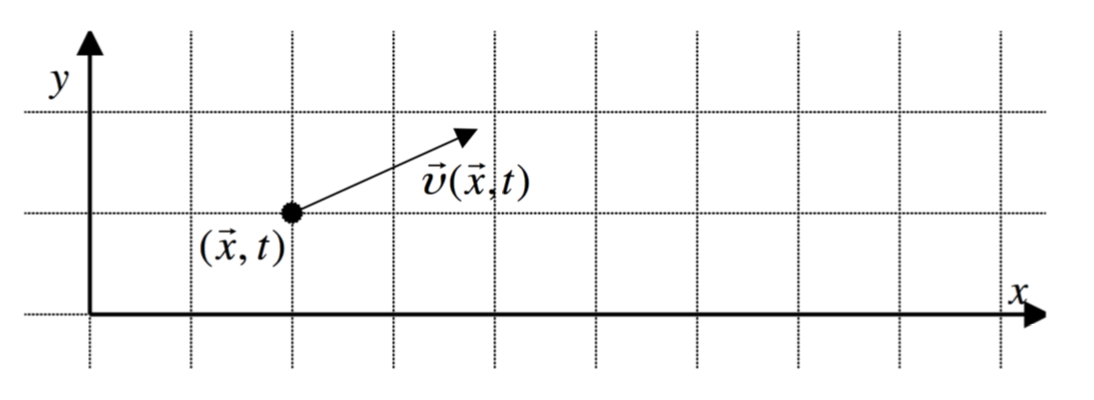
\includegraphics[scale = 0.4]{Figures/grid_method.png}
        \caption{Grid description, \textit{retrieved from MIT}(2011)}
    \end{figure}

\section{Smoothed Particle Hydrodynamics}
    Smoothed particle hydrodynamics (SPH) was invented to simulate nonaxisymmetric phenoma in astrophysis initially \cite{DBLP:journals/corr/GuWKMSSLWW15}. The principal idea of SPH is to treat hydrodynamics in a completely mesh-free fashion, in terms of a set of sampling particles. It turns out that the particle presentation of SPH has excellent conservation properties. Energy, linear momentum, angular momentum, mass and velocity.

    \subsection{Fundamentals}

    At the heart of SPH is a kernel interpolation method which allows any function to be expressed in terms of its values at a set of disordered points - the particles\cite{monaghan1992smoothed}. For ant field $A(\textbf{r})$, a smoothed interpolated version $A_{I}(\textbf{r})$ can be defined by a kernel $W(\textbf{r}, h)$,
    \begin{equation}
        A_{I}(\textbf{r}) = \int A({\textbf{r}}^{\prime})W(\|\textbf{r} - \textbf{r}^{\prime}\|, h)\dif\textbf{r}^{\prime}
    \end{equation}
    \begin{figure}[!ht]
        \centering
        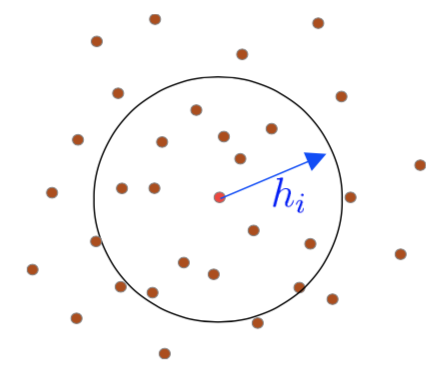
\includegraphics[scale = 0.6]{Figures/sph}
        \caption{Visilaztion of SPH}
    \end{figure}

    where the integration is over the entire space, and $W$ is an interpolating kernel with 
    \begin{equation}
        \int W(\|\textbf{r} - \textbf{r}^{\prime}\|, h)\dif \textbf{r}^{\prime} = 1
    \end{equation}
    and
    \begin{equation}
        \lim_{h\to 0} W(\|\textbf{r} - \textbf{r}^{\prime}\|, h)\dif\textbf{r}^{\prime} = \delta(\|\textbf{r} - \textbf{r}^{\prime}\|) 
    \end{equation}

    Normally, we want the kenel to be Non-negative and rotational invariant.
    \begin{equation}
        W(\|\textbf{x}_{i} - \text{x}_{j}\|, h) = W(\|\text{x}_{j} - \text{x}_{i}\|, h)
    \end{equation}

    \begin{equation}
        W(\|\textbf{r} - \textbf{r}^{\prime}\|, h) \ge 0
    \end{equation}

    For numerical work, we can use midpoint rule,
    \begin{equation}
        A_{I}(\textbf{x}) \approx A_{S}(\textbf{x}) = \sum_{i} A(\textbf{x}_{i})W(\|\textbf{x}_{i}-\textbf{x}\|, h)\Delta V_{i}
    \end{equation}
    Since $V_{i} = m_{i}/\rho _{i}$
    \begin{equation}
        A_{S}(\textbf{x}) = \sum_{i} \frac{m_{i}}{\rho_{i}} A(\textbf{x}_{i})W(\|\textbf{x}_{i}-\textbf{x}\|, h)
    \end{equation}

    The default, gradient and Laplacian of $A$ are:
    \begin{equation}
        \begin{aligned}
            \nabla A_{S}(\textbf{x}) &= \sum_{i} \frac{m_{i}}{\rho_{i}} A(\textbf{x}_{i})\nabla W(\|\textbf{x}_{i}-\textbf{x}\|, h) \\
            \nabla^{2} A_{S}(\textbf{x}) &= \sum_{i} \frac{m_{i}}{\rho_{i}} A(\textbf{x}_{i})\nabla^{2} W(\|\textbf{x}_{i}-\textbf{x}\|, h)
        \end{aligned}
        \label{eq:1}
    \end{equation}

    \subsection{Kernels}
    Smoothing kernels functions are one of the most important points in SPH. Stability, accurancy and speed of the whole method depends on these fuctions. Different kernels are being used for different purposes. One possibilyty for $W$ is a Gaussian. However, most current SPH implementations are based on kernels with finite support. We mainly introduce gaussian, poly6 and spicky kernel here. And compare the different kernels and their property.

    \subsubsection{Poly6}
    The kernel is also known as the 6th degree polynomial kernel.
    \begin{equation}
        W_{poly 6}(\textbf{r}, h) = \frac{315}{64\pi h^{9}}
            \begin{cases}
                (h^2 - \|\textbf{r}\|^2)^3 & 0 \le \|\textbf{r}\| \le h \\
                0 & \textrm{Otherwise}
            \end{cases}
    \end{equation}

    Then, the gradient of this kernel function can be
    \begin{equation}
        \nabla W_{poly 6}(\textbf{r}, h) = - \frac{945}{32\pi h^9}
            \begin{cases}
                \textbf{r}(h^2 - \|\textbf{r}\|^2)^2 & 0\le\|\textbf{r}\|\le h \\
                0 & \textrm{Otherwise}\\
            \end{cases}
    \end{equation}

    The laplacian of this kenel can be expressed by, 
    \begin{equation}
        \nabla^2 W_{poly6}(\textbf{r}, h) = - \frac{945}{16\pi h^9}
            \begin{cases}
                (h^2 - \|\textbf{r}\|^2)(3h^2-7\|\textbf{r}\|^2) & 0\le\|\textbf{r}\|\le h \\
                0 & \textrm{Otherwise}\\
            \end{cases}
    \end{equation}

    As M\"uller stated\cite{muller2003particle}, if the kernel is used for the computation of pressure forces, particles tend to build cluster under high pressure because `as particles get very close to each other, the repulsive force vanishes because the gradient of the kerbek approaches zero to the center.', which we can see in Figure \ref{fg:gradient}. Another kernel, spiky kernel, is proposed by Desbrum and Gascuel\cite{desbrun1996smoothed} to solve this problem.

    \subsubsection{Spicky}

    The kernel proposed by Desbrum and Gascuel\cite{desbrun1996smoothed}
    \begin{equation}
        W_{spiky}(\textbf{r}, h) = \frac{15}{\pi h^6}
            \begin{cases}
                (h - \|\textbf{r}\|)^3 & 0\le\|\textbf{r}\|\le h \\
                0 & \textrm{Otherwise}\\
            \end{cases}
    \end{equation}

    Then, the gradient of spiky kernel can be described by,
    \begin{equation}
        \nabla W_{spiky}(\textbf{r}, h) = -\frac{45 \textbf{r}}{\pi h^6 \|\textbf{r}\|}
            \begin{cases}
                (h - \|\textbf{r}\|)^2 & 0\le\|\textbf{r}\|\le h \\
                0 & \textrm{Otherwise}\\
            \end{cases}
    \end{equation}
     The laplacian of spiky can be expressed by,
     \begin{equation}
        \nabla^2 W_{spiky}(\textbf{r}, h) = \frac{90}{\pi h^6}
            \begin{cases}
                h - \| \textbf{r} \| & 0 \le \| \textbf{r} \| \le h \\
                0 & \textrm{Otherwise}\\
            \end{cases}
    \end{equation}

    \begin{figure}[!ht]
        \centering
        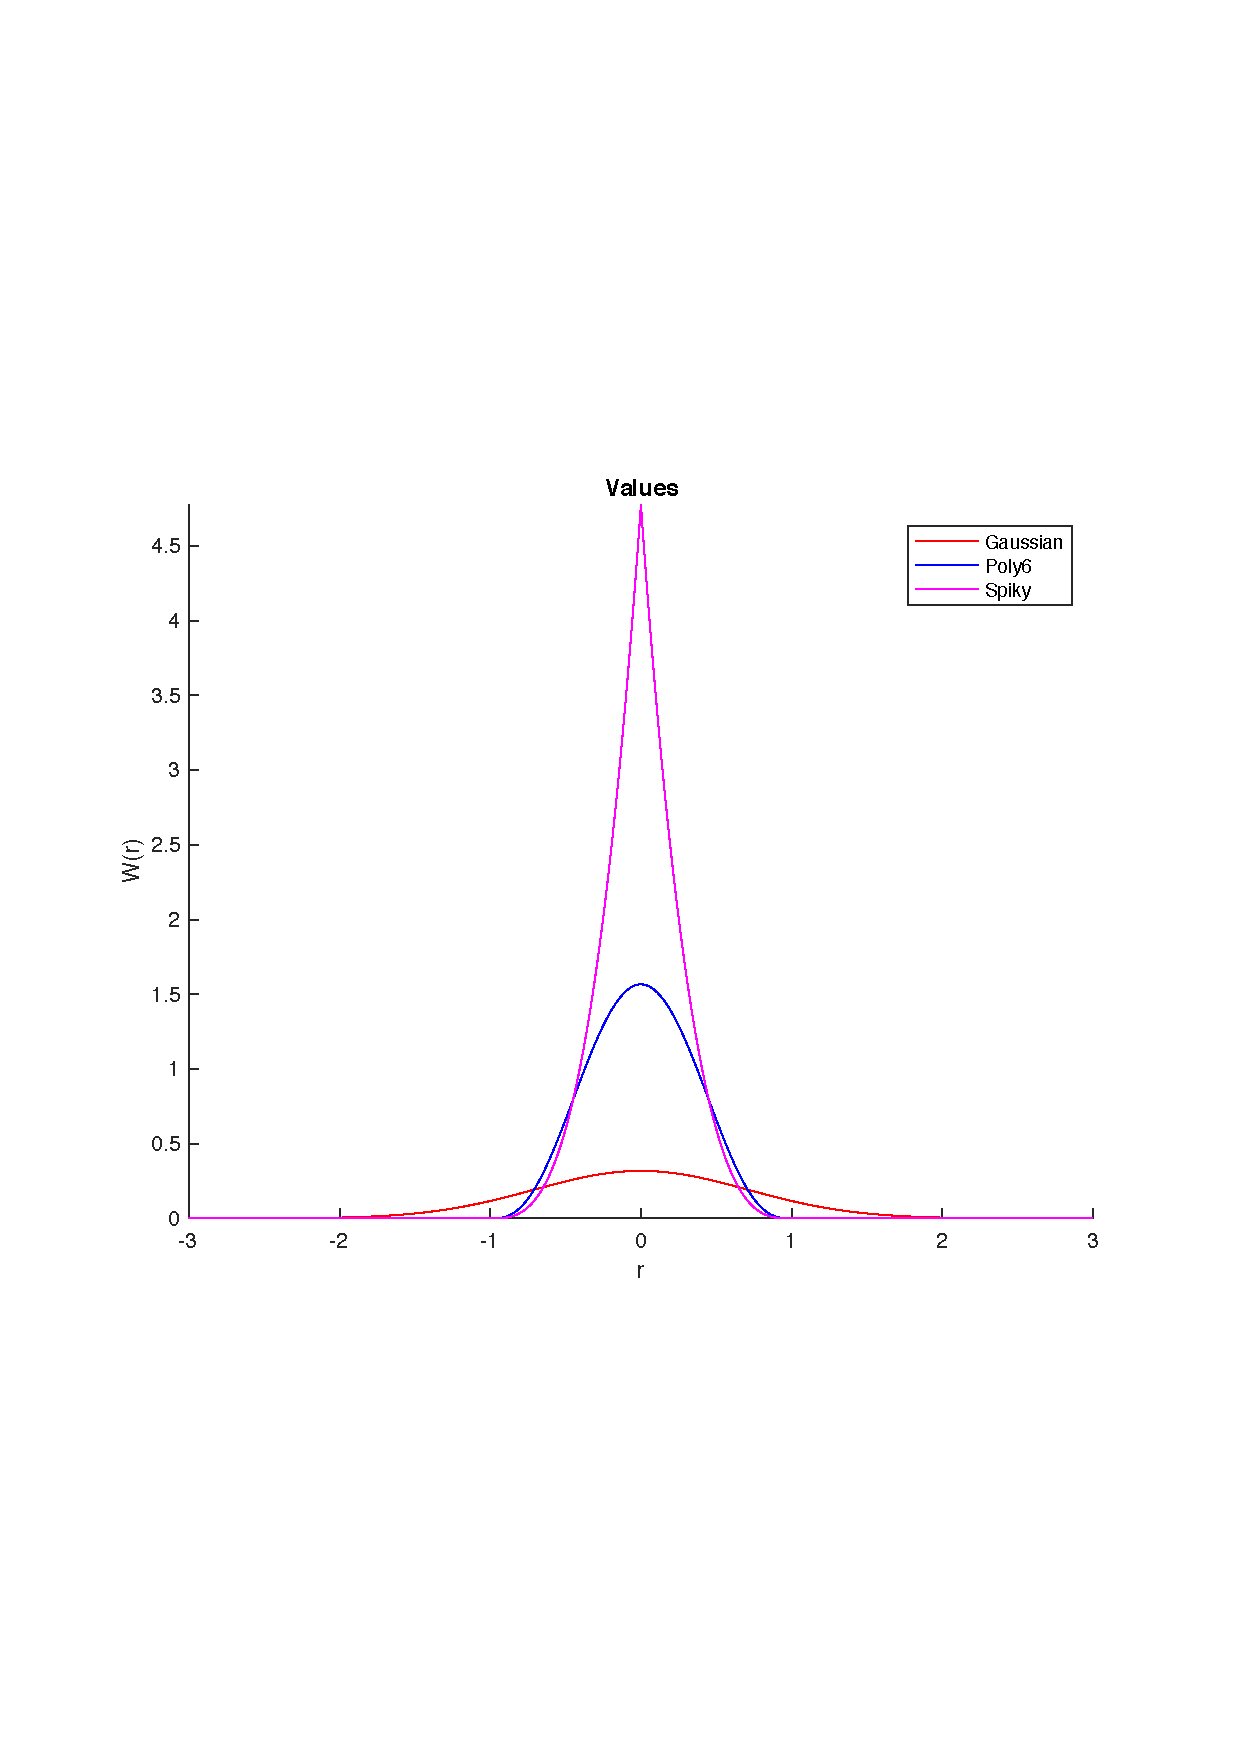
\includegraphics[scale = 0.5]{Figures/kernels}
        \caption{Comparation of different kernels, we set smoothing length $h = 1$ here.}
    \end{figure}

    \begin{figure}[!ht]
        \centering
        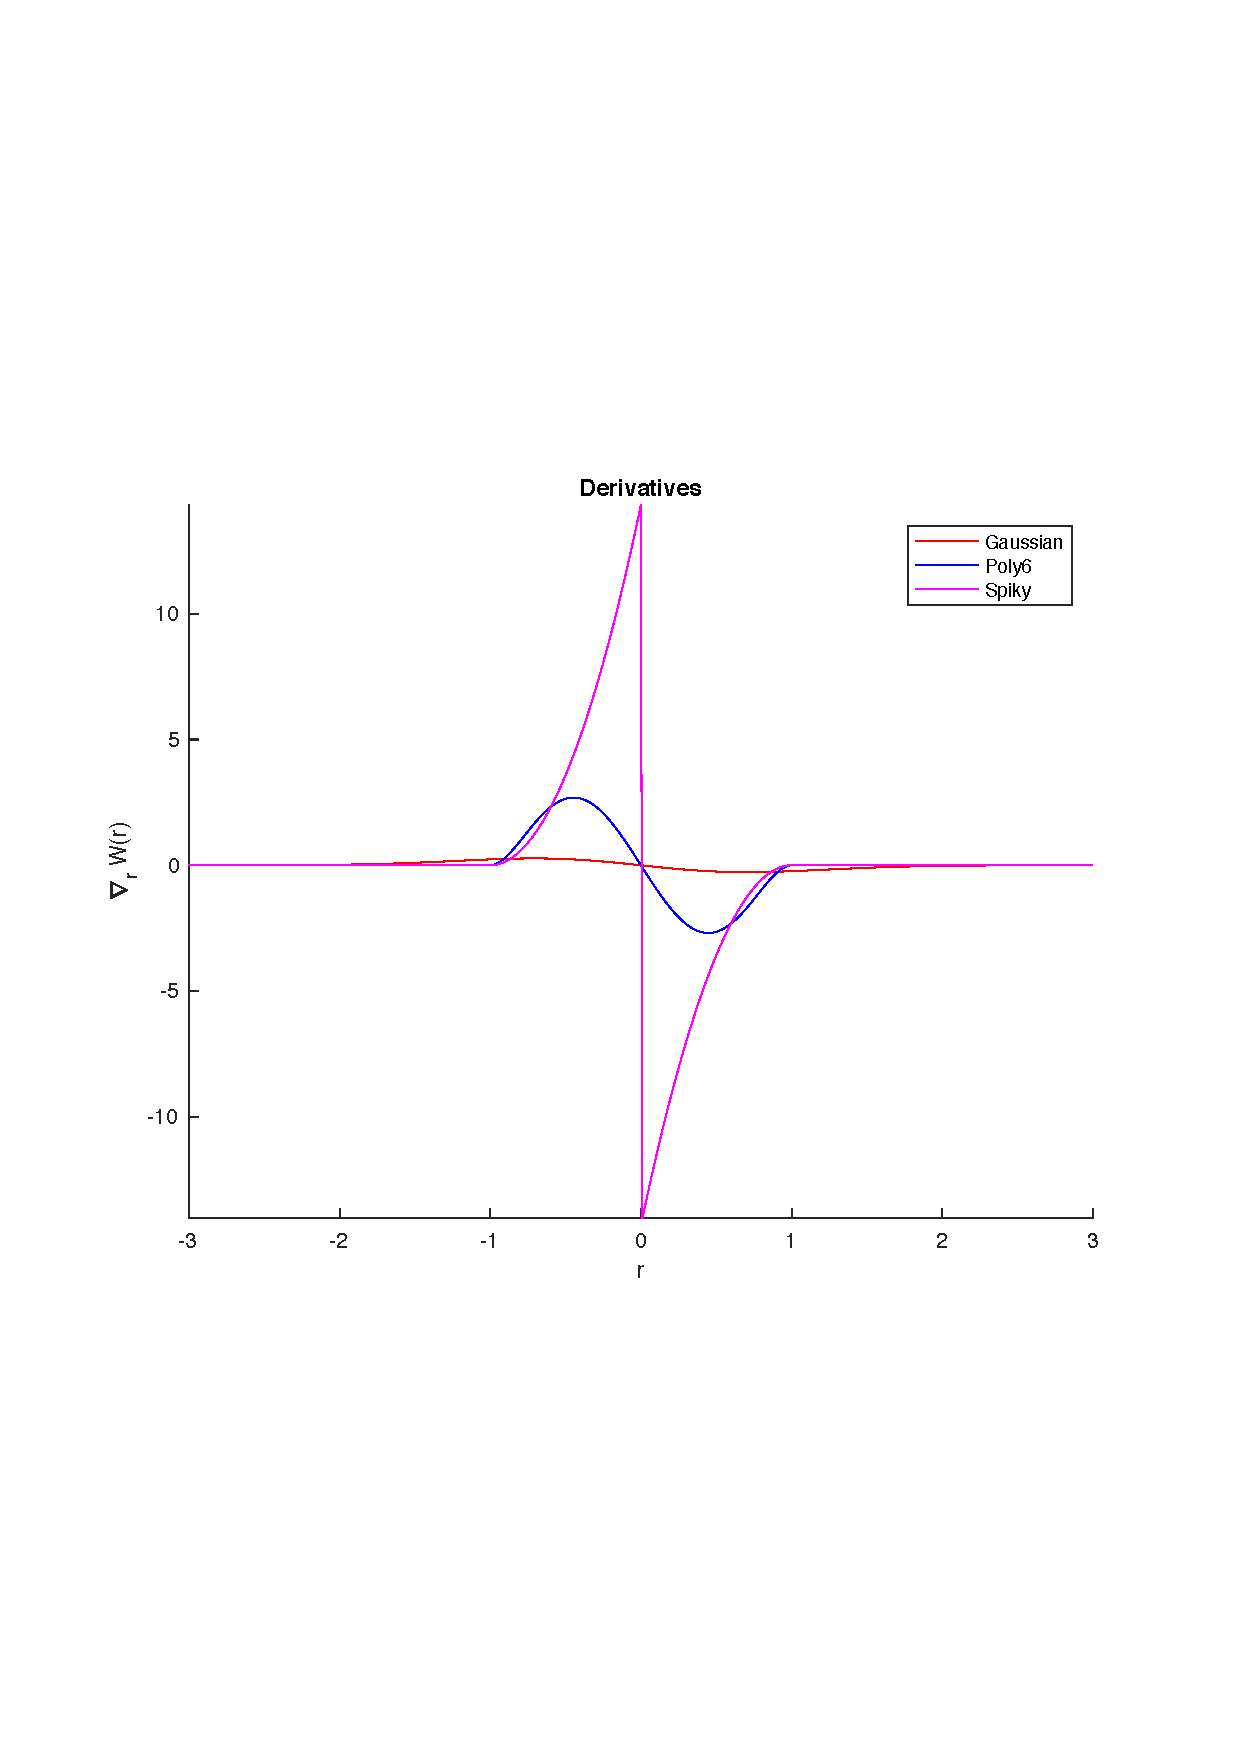
\includegraphics[scale = 0.5]{Figures/kenels_de}
        \caption{Comparation of gradient of different kernels, we set $h = 1$ here. }
        \label{fg:gradient}
    \end{figure}

    \subsection{Grid size and smoothing length}

    The grid should be also fine enough to capture the variation in our simulation. In our case, it is reasonable to have a grid fine enough such that no two contact points are mapped into the same cell. \\

    Smoothing length, $h$, is one of the most important parameters that affects the whole SPH method by changing the kernel value results abd neighbor searching results. Too small or too big values might cause lose essencail information in the simulation.

    \subsection{Neignbor Search}
    Neighbor search is one of the most crucial procedures in SPH method considersing all interpolation equations, $A(\textbf{r})$, needs the neighbor list for every particle (refer to equation \ref{eq:1}). A naive neighbor searching approach would end up with a complexity of $o(n^2)$. The complexity is not good enough since it is impossoble to reach any interactive speed when the particle count increses. With an efficient nearest neighbor searching(NNS) algorithm, it is possible to have a significant performance increase since it is the most time consuming procedure in SPH computation. In order to decrease the complexity, we choose to use $k-d$ tree data structure to store the particla spatial information and then do the nearest neighbor searching.

        \subsubsection{Hierarchical Tree}
        Using an adaptive hierarchy tree search is proposed by Paiva\cite{paiva2006particle} to find particle neighbors. Since the simulation takes place in two dimensions, $k-d$ tree data structure was used in this approach. \\

        An octree structure has been adapted from Macey (b) Octree Demo. The hierarchy tree is formed with a pre-defined height. The simulation box is divided recursively into eight pieces, nodes. The nodes at height = 1 are called leaves. Each node has a surrounding box for particle query which is used to check if the particle is inside the node. Each parent node, contains the elements that are divided through its children. The particle is being checked at each level of the tree if it’s intersecting the node. If it does, descend one level down in that node. After reaching to leaves, bottom level, particle has been checked if its within the search distance, $h$. If the particle is in the range, add it to the neighbor list. Neighbor searching is done when the whole tree has been traversed. The search distance set to be smoothing length in this implementation. \\

        The complexity of this tree search method is $O(nlog(n))$, n being the number of particles. The performance of this algorithm is worse than Spatial Hashing method. In addition, the results obtained using this NNS algorithm wasn’t accurate and stable for this implementation. Therefore as mentioned above, Spatial Hashing method was preferred.


\section{Grid to particle}
    SPH will be used for us to transform current state of dynamic system to grid images. After getting the grid image for simulation state in time $t$, we will use the grid cells as input and renew the contact grid image based on trained model. Once the contact force image is obtained, we will use contact position to interpolate image values. The interpolated values will be stored in the contact points and used as starting iterates for contact force solver. Then we can update states of all rigid bodies in time $t+\Delta{t}$.

    \subsection{Bilinear interpolation}
    We applied bilinear interpolation in our case, since we did mainly research on a rectilinear $2-D$ grid.
    \begin{figure}
        \centering
        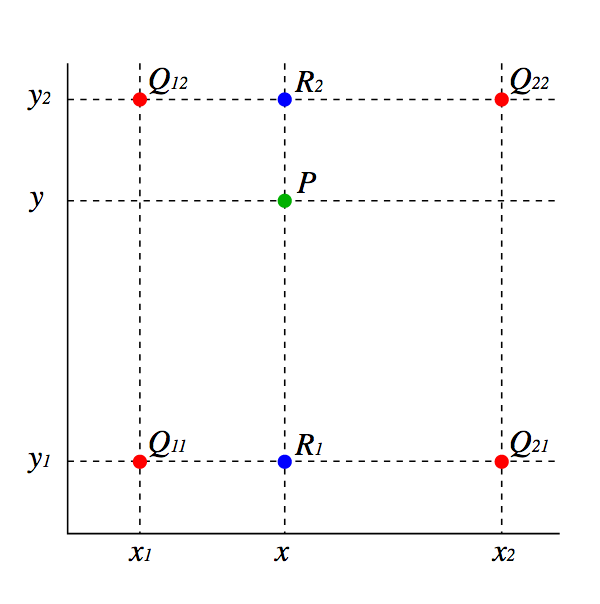
\includegraphics[scale = 0.8]{Figures/inp}
        \caption{The figure shows visiualization of bilinear interpolation. The four red dots show the data points and the green dot is the point at which we want to interpolate.}
        \label{fig:1}
    \end{figure}
    The key idea is to perform linear interpolation first in one direction, and then again in the other direction. Although each step is linear in the sampled values and in the position, the interpolation as a whole is not linear but rather quadratic in the sample location. \\

    As shown in Figure \ref{fig:1}, We have known $Q_{a, b} = (x_a, y_ b)$ and $a\in\{1, 2\}\quad b\in\{1,2\}$. Then, we can firstly do linear interpolation in the $x$-direction. This yields

    \begin{equation}
        \begin{aligned}
            f(x,y_{1})&\approx {\frac {x_{2}-x}{x_{2}-x_{1}}}f(Q_{11})+{\frac {x-x_{1}}{x_{2}-x_{1}}}f(Q_{21}),\\f(x,y_{2})&\approx {\frac {x_{2}-x}{x_{2}-x_{1}}}f(Q_{12})+{\frac {x-x_{1}}{x_{2}-x_{1}}}f(Q_{22}).
        \end{aligned}
        \label{eq:2}
    \end{equation}

    After getting the two values in $x-$direction $f(x, y_1)$ and $f(x, y_2)$, we can use these values to do interpolation in $y-$ direction.
    \begin{equation}
        f(x,y) \approx {\frac {y_{2}-y}{y_{2}-y_{1}}}f(x,y_{1})+{\frac {y-y_{1}}{y_{2}-y_{1}}}f(x,y_{2})
    \end{equation}

    Combine $f(x, y_1)$ and $f(x, y_2)$ defined in equation \ref{eq:2}, we can get,

    \begin{equation}
        \begin{aligned}
        f(x,y)&\approx{\frac {y_{2}-y}{y_{2}-y_{1}}}\left({\frac {x_{2}-x}{x_{2}-x_{1}}}f(Q_{11})+{\frac {x-x_{1}}{x_{2}-x_{1}}}f(Q_{21})\right)\\&\qquad+{\frac {y-y_{1}}{y_{2}-y_{1}}}\left({\frac {x_{2}-x}{x_{2}-x_{1}}}f(Q_{12})+{\frac {x-x_{1}}{x_{2}-x_{1}}}f(Q_{22})\right)\\&={\frac {1}{(x_{2}-x_{1})(y_{2}-y_{1})}}{\big (}\\&\qquad f(Q_{11})(x_{2}-x)(y_{2}-y)+f(Q_{21})(x-x_{1})(y_{2}-y)\\&\qquad+f(Q_{12})(x_{2}-x)(y-y_{1})+f(Q_{22})(x-x_{1})(y-y_{1}){\big )}\\&={\frac {1}{(x_{2}-x_{1})(y_{2}-y_{1})}}{\begin{bmatrix}x_{2}-x&x-x_{1}\end{bmatrix}}\\&\qquad \cdot {\begin{bmatrix}f(Q_{11})&f(Q_{12})\\f(Q_{21})&f(Q_{22})\end{bmatrix}}{\begin{bmatrix}y_{2}-y\\y-y_{1}\end{bmatrix}}
        \end{aligned}
        \label{interpolation}
    \end{equation}

\section{Experiment and Conclution}
    \label{sec:sph-exp}
    Our hope is that strating iterates will be close to ``solution'' of the contact problem, which can indicate the contact force solvers will coverage very rapidly or maybe not even need to iterate. In order to test whether the sph method can be applied in our case, the contact force solution is mapped to image and interpolated values are generated and used to restart the contact force solver. Our hyposis is that iterative solver quickly recovers an iteration close to the original solution before mapping to force grid image. I will just compare the performance of sph-based method with other methos in this section. More details will be analized and described in Chapter \ref{details}.

\subsection{pybox2d simulation}
    \label{sph:exp}
    In order to test whether \textbf{SPH-based} method works for this case. All experiments will be done based on the basis physical engine, \textit{pybox2d}. Before testing the performance of \textbf{SPH-based} method, \textbf{Non-model}, \textbf{Builtin-model} and \textbf{Copy-model} are defined to see the influence of different initial values for iterative contact solver.
    \begin{itemize}
        \item \textbf{Non-Model} In each step of the simulation, before the contact solver starts iteration to make resolution for current dynamic system equation, the initial $\lambda_{f}$ abd $\lambda_{t}$ of every contact will be given value $0$.
        \item \textbf{Builtin-Model} In each step of the simuation, before the contact solver starts iterations to make resolution for current dynamic state equation, the initial value of $\lambda_f$ and $\lambda_{t}$ will be determined by built-in algorithm. In other words, this model is default solution built in \textit{pybox2d}.
        \item \textbf{Copy-Model} In each step of simulation, before the contact solver starts iteration to make resolution for current dynamic system equation, the initial value of $\lambda_f$ and $\lambda_t$ will be the actual solution after exact iterations sover.
    \end{itemize}
    After defining these models, each model will be applied in the same rigid dynamic simulation process. The setting is given below,
    \begin{itemize}
        \item \textbf{World Setting}, the world box size is $30\times30$,   and there are $100$ circle rigids($r=1$, all circle rigid bodies in the same size.) inside the box. Initially, the rigid circles will be located following gaussian distribution\footnote{\url{https://en.wikipedia.org/wiki/Normal_distribution}}. Then, all rigid circles will fall down by gravity. The visualization of simulation is shown in Figure \ref{fig:simvi}.
        \item \textbf{Simulation Setting}, there will be totally $600$-steps simulation. For each step, $\Delta t = 0.01s$, and the number of iteration in  eacg step will be set as fixed, $3000$. Then I will use the average covergence rate to show how fast the model coverages.
    \end{itemize}
    \begin{figure}[!h]
        \centering
        \begin{subfigure}[b]{0.3\textwidth}
            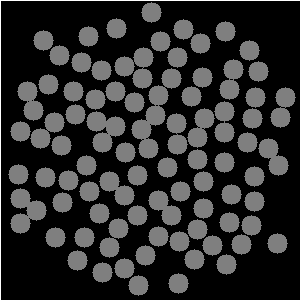
\includegraphics[width=\textwidth]{Figures/sim0.png}
            \caption{Time Step=$0$}
        \end{subfigure}
        \begin{subfigure}[b]{0.3\textwidth}
            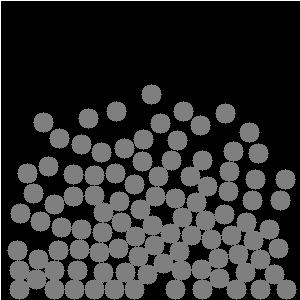
\includegraphics[width=\textwidth]{Figures/sim2.png}
            \caption{Time Step=$200$}
        \end{subfigure}
        \begin{subfigure}[b]{0.3\textwidth}
            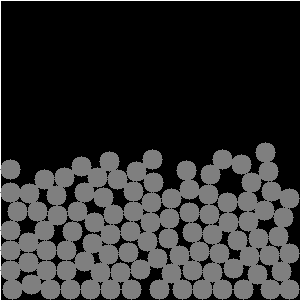
\includegraphics[width=\textwidth]{Figures/sim3.png}
            \caption{Time Step=$400$}
        \end{subfigure}
        \caption{Visualization for experiment simulation}
        \label{fig:simvi}
    \end{figure}
    \begin{figure}[!h]
        \centering
        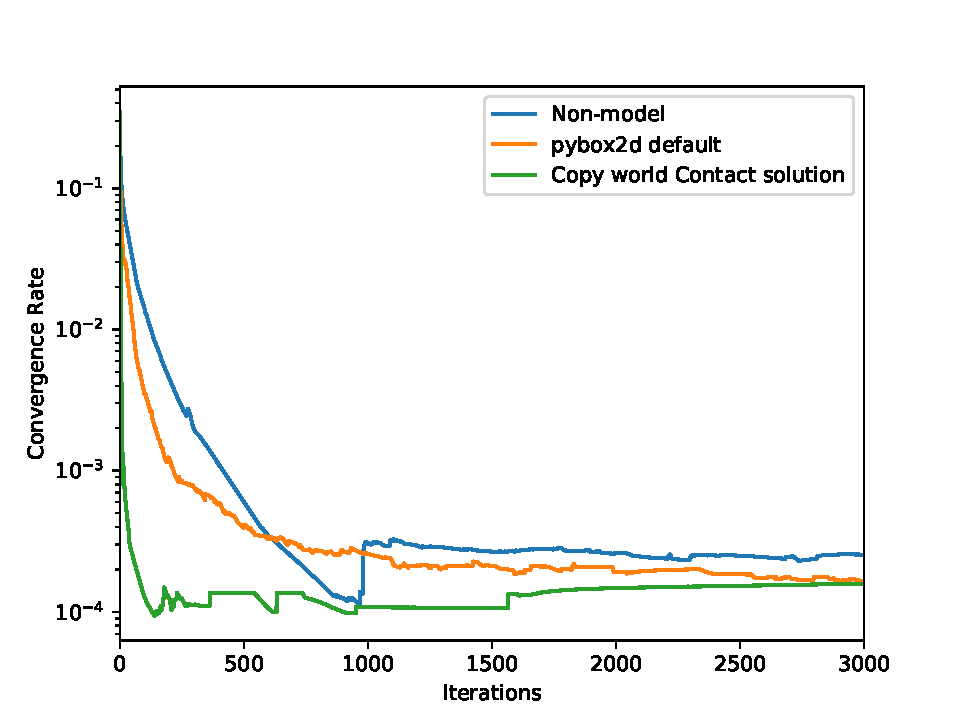
\includegraphics[width=\textwidth]{Figures/nosph}
        \caption{Average covergence rate for different models(not including \textbf{SPH-based model}).}
        \label{fg:nosph}
    \end{figure}
    The results are described in Figure \ref{fg:nosph}. Obviously, \textbf{Copy-Model} performs the best, coverages the most rapidly. Once all the initial values for iterative solver are zero, it has to take long time to reach converagence, which is indicated by \textbf{Non-Model}. The \textbf{Builtin-Model} get converagence much fater than \textbf{Non-Model}, but still slower than \textbf{Copy-Model}. Then one hypothesis about sph based method can be,
    \begin{itemize}
        \item The performance of \textbf{SPH-Model} will converge similar to \textbf{Builin-Model}, even better.
    \end{itemize}

\subsection{SPH-based method test}
    The \textbf{SPH-Model} is defined as follow, as well as the experiment algorithm in \ref{testsph},
    \begin{itemize}
         \item \textbf{SPH-Model} In each step of simulation, one grid map $G(\mathbf{\pmb{\lambda}})~~\pmb{\lambda} = [\lambda_n, \lambda_t]$ will be created based on given rigid bodies $\mathcal{B}$ and contacts $\mathcal{C}$ between the bodies. Then, interpolated values will be generated by given contact point position $(x_j, y_j)~~j \in \mathcal{C}$ and will be used as initial values for iterative contact solver in \textit{pybox2D}. 
    \end{itemize}
    \begin{algorithm}[!h]
        \KwData{
            Given a set of bodies $\mathcal{B}$ and the state in time $t$, as well as some information of contacts between these bodies $\mathcal{C}$.
        }
        \KwResult{Get the contact forces $\pmb{\lambda}_{j}=[{\lambda_{n}}_{j}, {\lambda_{t}}_j]~~j\in\mathcal{C}$ at time $t$.}
        \While{Simulation Runing}
        {
            1. read current state,
                $$\pmb{\lambda}_{j}=[{\lambda_{n}}_{j}, {\lambda_{t}}_{j}]~~j\in\mathcal{C}$$ \\
            2. map the solved contact to a gird image, $\mathbf{x}=(x_i, y_i)$ is the spatial position of one node in in grid image.
                $$G_{\pmb{\lambda}}(\mathbf{x}) \equiv \sum_{j \in \mathcal{C}} W(\mathbf{x}, \pmb{q}_{j})\pmb{\lambda}_{j},~~\pmb{\lambda}=[\lambda_n, \lambda_t]$$ \\
            3. Once the contact force image is obtained,  the conatct position $\pmb{q}_{j} = (x_{j}, y_{j})~~j\in\mathcal{C}$  will be used to interpolation image values based on Equation \ref{interpolation}.
                $$\pmb{\lambda}_j \approx G_{\pmb{\lambda}}(\pmb{q}_j)~~j\in\mathcal{C}$$ 
            The interpolated values $\pmb{\lambda}$ will be used as restarting iterated for \textit{pybox2d} conatc solver. \\
            4. Update $t$
                $$t = t + \Delta t$$ \\
        }
        \caption{Experiment algorithm for test \textbf{SPH-Model}}
        \label{testsph}
    \end{algorithm}
     \begin{figure}
        \centering
        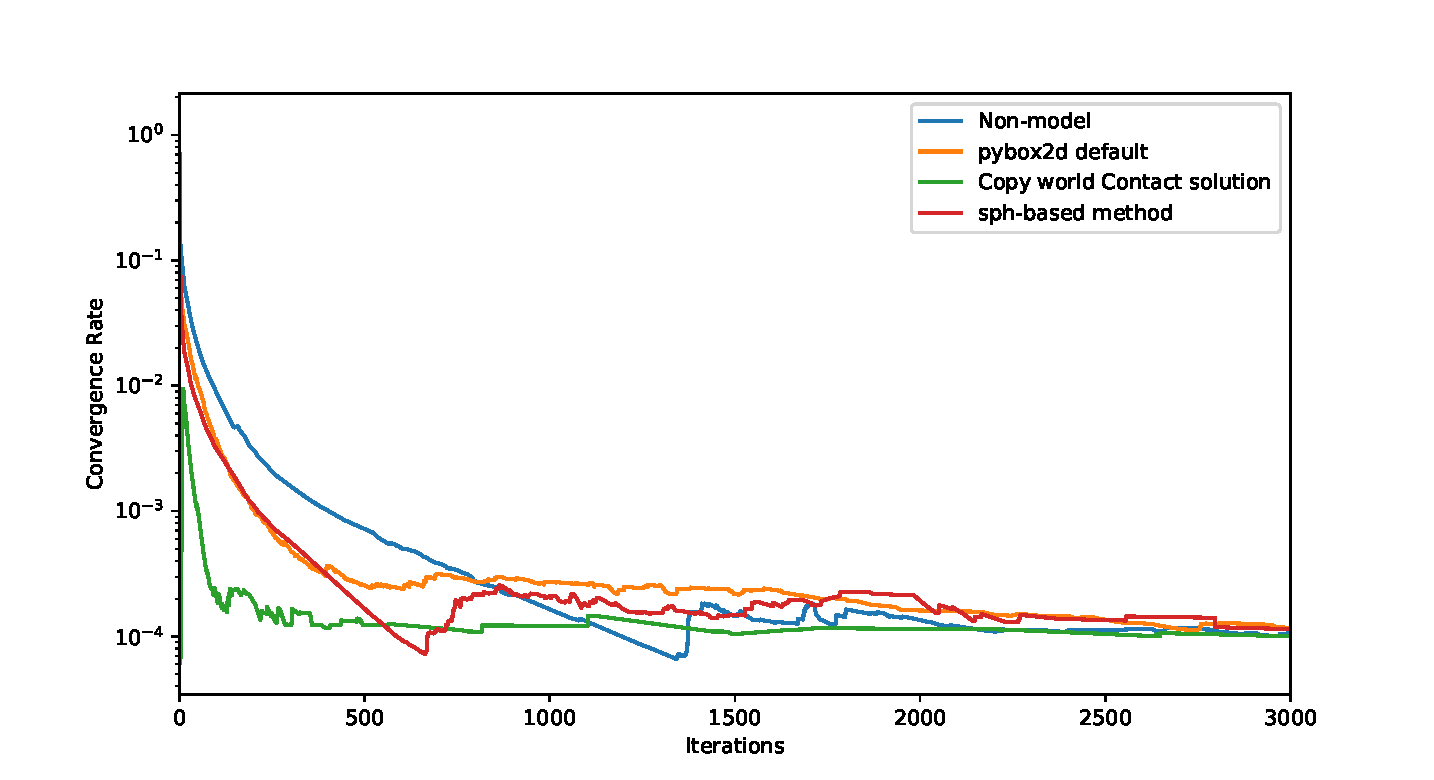
\includegraphics[width=\textwidth]{Figures/addsph}
        \caption{Covergence rate for different models(including \textbf{SPH-based model}).}
        \label{fg:addsph}
    \end{figure}
    As the hypothesis we expect, \textbf{SPH-Model} converages even faster than \textbf{builtin-Model}. This can demonstrade the \textbf{sph-based} method is a good strategy, which can make itervative contact solver coverage quickly.
\subsection{Conlusion}
    Based the result in Figure \ref{fg:nosph} and \ref{fg:addsph}, it can be concluded that \textbf{SPH-based} strategy is available for the case in this thesis. Once the correct contact forces grid is acheived, the interpolated values will help the iterative solver to get convergence faster. So, the next step is to train a suitable model based on training data. The overall algorithm is concluded in Algorithm \ref{al:basic}.
    \begin{algorithm}[!h]
        \KwData{
            Given a set of bodies $\mathcal{B}$ and the state in time $t$, as well as some information of contacts between these bodies $\mathcal{C}$.
        }
        \KwResult{Get the contact forces $\pmb{\lambda}_{j}=[{\lambda_{n}}_{j}, {\lambda_{t}}_j]~~j\in\mathcal{C}$ at time $t$.}
        \While{Simulation Runing}
        {
            1. read current state, $\mathbf{x}=(x_i, y_i)$ is the spatial position of one node in in grid image.
                $$m_i, \pmb{v}_i, \pmb{q}_i, \omega_{i}~~i\in\mathcal{B}$$
                $$\pmb{n}_j~~j\in\mathcal{C}$$ \\
            2. map the current state to a gird image,
                $$G_{m}(\mathbf{x}) \equiv \sum_{i\in \mathcal{B}}W(\mathbf{x}, \pmb{q}_{i})m_i$$ 
                $$G_{\pmb{v}}(\mathbf{x}) \equiv \sum_{i\in \mathcal{B}}W(\mathbf{x}, \pmb{q}_{i})\pmb{v}_i,~~\pmb{v}=(v_x, v_y)$$
                $$G_{\pmb{n}}(\mathbf{x}) \equiv \sum_{i\in\mathcal{C}}W(\mathbf{x}, \pmb{q}_{i})\pmb{n}_{i},~~\pmb{n}=(n_x,n_y)$$
                $$G(\mathbf{x}) = [G_{m}(\mathbf{x}), G_{\pmb{v}}(\mathbf{x}), G_{\pmb{n}}(\mathbf{x})]$$ \\
            3. Use $G(\mathbf{x})$ as the input image to the learning model, the output will be resize to a imag, the output image will be called $G_{output}$,
                $$G_{output}(\mathbf{x}) = [G_{\lambda_{n}}(\mathbf{x}), G_{{\lambda}_{t}}(\mathbf{x})]$$ \\
            4. Once the contact force image is obtained,  the conatct position $\pmb{q}_{j} = (x_{j}, y_{j})~~j\in\mathcal{C}$  will be used to interpolation image values based on Equation \ref{interpolation}.
                $$\pmb{\lambda}_j \approx G_{output}(\pmb{q}_j)~~j\in\mathcal{C}$$ 
            The interpolated values $\pmb{\lambda}$ will be used as starting iterated for \textit{pybox2d} conatc solver. \\
            5. Update $t$
                $$t = t + \Delta t$$ \\
        }
        \caption{Introducrion to the deep contact model solver in this thesis.}
        \label{al:basic}
    \end{algorithm}

